
%(BEGIN_QUESTION)
% Copyright 2013, Tony R. Kuphaldt, released under the Creative Commons Attribution License (v 1.0)
% This means you may do almost anything with this work of mine, so long as you give me proper credit

This process flow diagram shows a Fluid Catalytic Cracking (FCC) unit, commonly found in oil refineries:

$$\includegraphics[width=15.5cm]{i03559x01.eps}$$

Given a ``heavy hydrocarbon'' feed flow rate of 75,000 barrels per day into this FCC unit, calculate the velocity of this oil exiting the feed pump if the discharge pipe on that pump is 8 inches in diameter:

\vskip 10pt

$v$ = \underbar{\hskip 50pt} feet per second

\vskip 20pt

Additionally, choose the \underbar{one} statement best describing the relative {\it boiling points} of the feed versus fractionator products in this FCC unit:

\begin{itemize}
\item{} HGO boils at a higher temperature than LGO, and LGO boils at a higher temperature than feed
\item{} HGO boils at a higher temperature than feed, and feed boils at a higher temperature than LGO
\item{} LGO boils at a higher temperature than HGO, and HGO boils at a higher temperature than feed
\item{} LGO boils at a higher temperature than feed, and feed boils at a higher temperature than HGO
\item{} Feed boils at a higher temperature than HGO, and HGO boils at a higher temperature than LGO
\item{} Feed boils at a higher temperature than LGO, and LGO boils at a higher temperature than HGO
\end{itemize}

\underbar{file i03559}
%(END_QUESTION)





%(BEGIN_ANSWER)

The volumetric flow rate for any fluid is equal to the flow velocity ($v$) multiplied by the cross-sectional area of the pipe ($A$):

$$Q = Av \hskip 30pt v = {Q \over A}$$

$$A = \pi r^2$$

$$A = \pi \left(8 \over 2 \right)^2 = 50.27 \hbox{ in}^2 = 0.349 \hbox{ ft}^2$$

$$\left(75000 \hbox{ bbl} \over \hbox{day} \right) \left(1 \hbox{ day} \over 24 \hbox{ hr} \right) \left( 1 \hbox{ hr} \over 3600 \hbox{ s} \right)  \left( 42 \hbox{ gal} \over 1 \hbox{ bbl} \right)  \left( 231 \hbox{ in}^3 \over 1 \hbox{ gal} \right)  \left( 1 \hbox{ ft}^3 \over 1728 \hbox{ in}^3 \right) = 4.874 \hbox{ ft}^3\hbox{/s}$$

$$v = {Q \over A} = {4.874 \hbox{ ft}^3\hbox{/s} \over 0.349 \hbox{ft}^2} = 13.96 \hbox{ ft/s}$$

\vskip 20pt

Feed boils at a higher temperature than HGO, and HGO boils at a higher temperature than LGO


%(END_ANSWER)





%(BEGIN_NOTES)


%INDEX% Process: fluid catalytic cracker (oil refinery)

%(END_NOTES)


